One of the simplest algorithms we have implemented is Dijkstra's algorithm
for the single source shortest paths problem.
Fig.~\ref{fig:dijkstra}
shows most of the implementation of the animation of Dijkstra's algorithm.
At every step the nodes already in the shortest path tree are \emph{visited}
(gray shading) and the nodes that have been encountered (but are not in the tree)
are \emph{selected }(thick red boundary).\footnote{
  Because these node and edge states both guide the logic of the algorithm
  and how the nodes/edges are displayed, the nomenclature has become awkward.
  A better way to handle the situation is to add initial declarations
  that specify color, thickness, and, in case of nodes, fill color, for each logical state.
  A logical state would have a name, e.g., \emph{InTree},
  and be automatically provided with a setter (Boolean argument),
  e.g., \emph{setInTree}, and a logical test, e.g., \emph{isInTree}.
}
Selected \emph{edges} (thick red) represent the current shortest paths to all
encountered nodes;
they are the edges of a shortest path tree when the algorithm is done.
The same algorithm animation
works for both directed and undirected graphs, as illustrated
in Figs.~\ref{fig:dijkstra_directed} and~\ref{fig:dijkstra_undirected}.
The user can toggle between the directed and undirected versions of a graph
via push of the appropriate button.
The functions \emph{beginStep} and \emph{endStep} define the points at which
the exploration of the algorithm stops its forward or backward motion.
In their absence, any state change (mark, select, change in weight, etc.)
constitutes a step, which, in some cases, can force the user
to do excessive ``stepping'' to move past uninteresting state changes.

\begin{figure}

\small
\begin{verbatim}
algorithm {
    NodePriorityQueue pq = new NodePriorityQueue();
    Edge [] chosenEdge = new Edge[nodeIds()]; 
    beginStep();
    for_nodes(node) {
        node.setWeight(INFINITY);
        pq.add(node);
    }
    Node v = getStartNode();
    setWeight(v, 0);
    endStep();

    while ( ! pq.isEmpty() ) {
        v = pq.removeMin();
        mark(v);        // nodes are marked when visited
        unHighlight(v); // and highlighted when on the frontier
        for_outgoing ( v, e, w ) {
            if ( ! marked(w) )  {
                if ( ! highlighted(w) ) highlight(w);
                double distance = weight(v) + weight(e);
                if ( distance < weight(w) ) {
                    beginStep();
                    highlight(e);
                    Edge previous_chosen = chosenEdge[id(w)];
                    if (previous_chosen != null )
                        unHighlight(previous_chosen);
                    pq.decreaseKey(w, distance);
                    chosenEdge[id(w)] = e;
                    endStep();
                }
            } // end, neighbor not visited (not in tree); do nothing if node
              // is already in tree
        } // end, adjacency list traversal
    } // stop when priority queue is empty
} // end, algorithm
\end{verbatim}

% \begin{verbatim}
% algorithm {
%     NodePriorityQueue pq = new NodePriorityQueue();
%     Edge [] chosenEdge = new Edge[nodeIds()]; 
%     beginStep();
%     for_nodes(node) {
%         node.setWeight(INFINITY);
%         pq.add(node);
%     }
%     Node v = getStartNode();
%     v.setSelected(true);
%     v.setWeight(0);
%     endStep();

%     while ( ! pq.isEmpty() ) {
%         v = pq.removeMin();
%         v.setVisited(true);
%         v.setSelected(false);
%         for_outgoing ( v, e, w ) {
%             if ( ! w.isVisited() )  {
%                 if ( ! w.isSelected() ) w.setSelected(true);
%                 double distance = v.getWeight() + e.getWeight();
%                 if ( distance < w.getWeight() ) {
%                     beginStep();
%                     e.setSelected(true);
%                     Edge previous_chosen = chosenEdge[id(w)];
%                     if (previous_chosen != null )
%                         previous_chosen.setSelected(false);
%                     pq.decreaseKey(w, distance);
%                     chosenEdge[id(w)] = e;
%                     endStep();
%                 }
%             } // end, neighbor not visited (not in tree); do nothing if node
%               // is already in tree
%         } // end, adjacency list traversal
%     } // stop when priority queue is empty
% } // end, algorithm
% \end{verbatim}

\caption{The implementation of the Dijkstra' algorithm animation.}
\label{fig:dijkstra}
\end{figure}


\begin{figure}[p]

\begin{center}
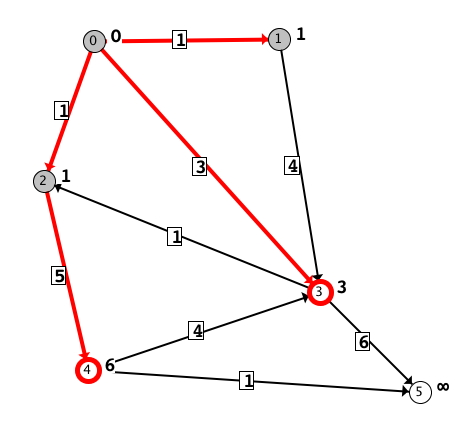
\includegraphics[scale=0.55]{X_dijkstra_directed}
\end{center}

\caption{Dijkstra's algorithm on a directed graph.}
\label{fig:dijkstra_directed}
\end{figure}


\begin{figure}[p]

\begin{center}
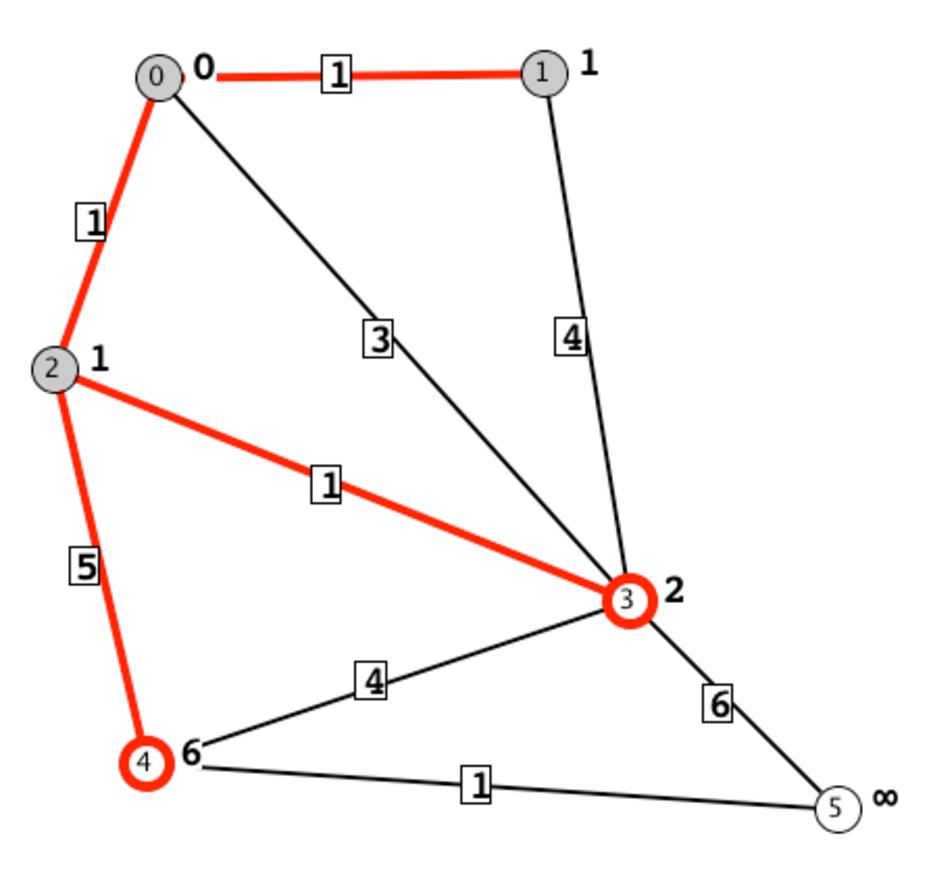
\includegraphics[scale=0.55]{X_dijkstra_undirected}
\end{center}

\caption{Dijkstra's algorithm on the same graph, undirected.}
\label{fig:dijkstra_undirected}
\end{figure}


The macro \emph{for\_outgoing($v,e,w$)}
creates a loop whose body is executed once
for each edge leading out of $v$; in the body, $e$ refers to the current edge
and $w$ to the other endpoint (any other variable names can be used).
In an undirected graph the term \emph{outgoing} applies to all incident
edges.\footnote{
Also provided are \emph{for\_incoming} and \emph{for\_adjacent};
the latter applies to all incident edges, even for directed graphs.
}

The difference between what the algorithm does on a directed versus an undirected graph is evident in the figures.
The edge \emph{from} node~3 to node~2 in the directed graph becomes an
edge \emph{between} the two nodes in the undirected form of the same graph.
Thus, in the undirected version, when node~2 is added to the tree
it also causes the distance from the source, node~0, to node~3 to be updated,
via the path through node~2.
These snapshots come from the executions of the \emph{same algorithm} on the
\emph{same graph}.
The only difference is that the explorer toggled from the directed to
the undirected
interpretation of the graph.
